\begin{figure}[H]
    \centering
    \begin{minipage}{0.33\textwidth}
        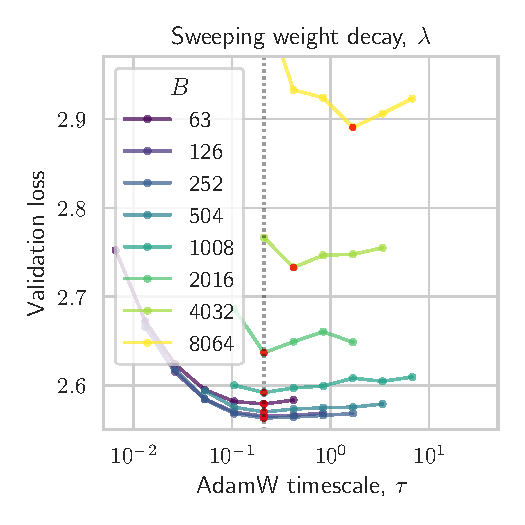
\includegraphics[trim={0.3cm 0.4cm 0.3cm 0.3cm}, clip, width=\linewidth]{pdffigs/loss_data.241005_batchsizes.617M.20tpp.D2Z.tepoch.sweep_wd.pdf}
    \end{minipage}\hfill
    \begin{minipage}{0.33\textwidth}
        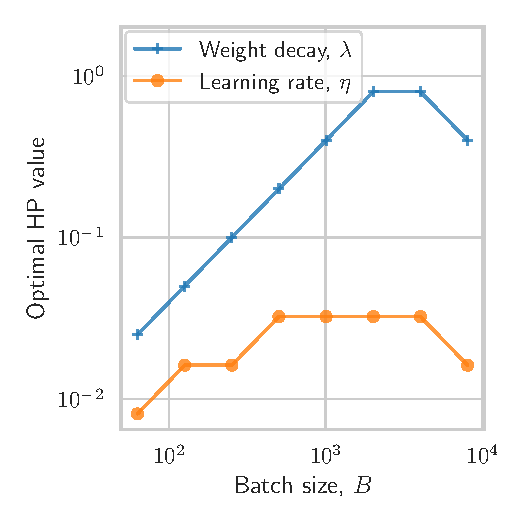
\includegraphics[trim={0.3cm 0.4cm 0.3cm 0.3cm}, clip, width=\linewidth]{pdffigs/loss_data.241005_batchsizes.lr_v_wd.617M.20TPP.pdf}
    \end{minipage}\hfill
    \begin{minipage}{0.33\textwidth}
        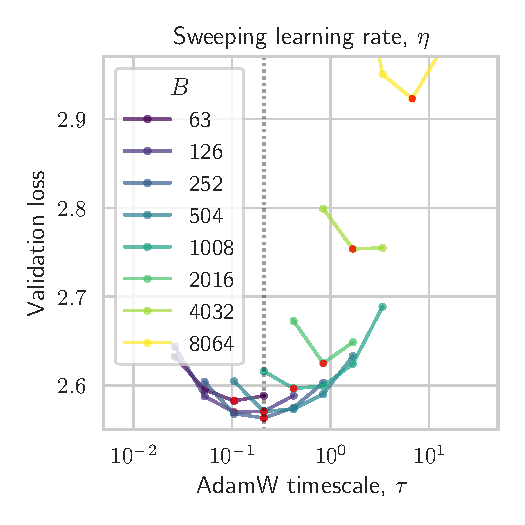
\includegraphics[trim={0.3cm 0.4cm 0.3cm 0.3cm}, clip, width=\linewidth]{pdffigs/loss_data.241005_batchsizes.617M.20tpp.D2Z.tepoch.sweep_lr.pdf}
    \end{minipage}
    \caption{(610M 20TPP): For each $B$, we sweep $\lambda$ and find
      $\tepochopt$ ($\leftfig$). $\tepochopt$ is stable around 0.21
      for $B \in [63, 2016]$, meaning $\lambdaopt$ scales linearly
      with $B$ over this range ($\middlefig$).  When sweeping $\eta$
      ($\rightfig$), the lower boundary over all curves is a bowl with
      a minimum at 0.21; the smallest $B$ settings have $\tepochopt$
      within 2$\times$ of this value, but as $B$ increases,
      $\tepochopt$ quickly drifts higher.\label{fig:tepochs}}
\end{figure}
